\documentclass[fleqn, oneside, 10pt, titlepage]{article}
%
%Zeichensatz UTF-8 und T1-Zeichensatz

\usepackage[utf8x]{inputenc} 
\usepackage[T1]{fontenc}
%Folgender Befehl verhindert pixelige Schrift
\usepackage{ae,aecompl}
\newcommand{\changefont}[3]{\fontfamily{#1}\fontseries{#2}\fontshape{#3}\selectfont}
% 

%Silbentrennung nach neuer deutscher Rechtschreibung
\usepackage[english]{babel} % Neue Rechtschreibung
%
%Einige Mathe-Symbole aus AMS-LaTeX
\usepackage{amsmath,amssymb,euscript}

\usepackage{algorithm2e}
%
% schönere Aufzählungen
\usepackage{enumerate}
%
% Für Bilder 
\usepackage{graphicx}

%Graue box
\usepackage{framed}
\usepackage{xcolor}

\definecolor{MyBoxColor}{rgb}{0.9,0.9,0.9}
\newenvironment{shadedSmaller}{
  \def\FrameCommand{\fboxsep=\FrameSep \colorbox{MyBoxColor}}
  \MakeFramed {\advance\hsize-2\width\FrameRestore}}
{\endMakeFramed}

\newenvironment{shadedSmallerPadding}{
  \def\FrameCommand{\fboxsep=0.3cm \colorbox{MyBoxColor}}
  \MakeFramed {\advance\hsize-1.1\width\FrameRestore}}
{\endMakeFramed}

%
% Farben und die Code-Umgebung einbinden
%
\usepackage{listings, color}
%
% Ein paar Standardfarben
\definecolor{darkblue}{rgb}{0,0,.6}
\definecolor{darkred}{rgb}{.6,0,0}
\definecolor{darkgreen}{rgb}{0,.6,0}
\definecolor{red}{rgb}{.98,0,0}
%
%Standardmäßig Java vorher laden
\lstloadlanguages{Java}
\lstloadlanguages{SQL}
% Standard-Layout für die Code-Umgebung (alle Sprachen)
\lstset{%
	language=SQL,
 	basicstyle=\normalsize\ttfamily,
	showspaces=false,
	showtabs=false,
	columns=fixed,
	frame=none,
	numberstyle=\tiny,
	breaklines=true,
	showstringspaces=false,
	xleftmargin=0cm,
	tabsize=4,
	keywordstyle=\color{darkblue},
	commentstyle=\color{darkred},
	stringstyle=\color{darkgreen},
	emph={i, t, a, f},
	emphstyle=\color{red}
}%

%
% Seitenranddefinitionen
%   Links etwas mehr Rand als rechts, damit sich die Zettel später besser abheften lassen.
\usepackage[a4paper]{geometry} 
\geometry{a4paper,tmargin=2.5cm, bmargin=3cm, lmargin=3cm, rmargin=2cm, headheight=3em, headsep=1em, footskip=1cm} 

%
% Kopf- und Fußzeilendefinition
%
\usepackage{fancyhdr}
\pagestyle{fancy}
\fancyhf{}
%
% Oben rechts die Namen der Teilnehmer der Gruppe
\fancyhead[R]{%
\textcolor{gray}{Andreas Rain}}
%
%Oben Links das Fach und darunter die Nummer des Übungsblattes
\fancyhead[L]{\textcolor{gray}{Data mining \\ Summarization}}
%
% Die Übungsgruppe oben in der Mitte (momentan auskommentiert)
%\fancyhead[C]{\changefont{pag}{m}{n} \textcolor{gray}{T = Do, 12-14 Uhr}}
%
%Fußzeile mittig die Seitenzahl
\fancyfoot[C]{\textcolor{gray}{Seite \thepage}}
%
% Fußzeile links das aktuelle Datum (alternativ kann hier der Abgabetag eingetragen werden)
\fancyfoot[L]{\textcolor{gray}{\today}}

%Fancy Table
\usepackage{tabularx}
\usepackage{booktabs}
\usepackage{colortbl}
\usepackage{tikz}
\usetikzlibrary{calc}
\pgfdeclarelayer{background}
\pgfdeclarelayer{foreground}
\pgfsetlayers{background,main,foreground}
%

%
% Deutsche Absatzformatierung: Zwischen zwei Absätzen eine Zeile (1em) frei und 
% kein Einrücken der ersten Zeile
%
\setlength{\parskip}{1em}
\setlength{\parindent}{0pt}

%
%Anktiviere die Paragraphen-Nummernanzeige
\setcounter{secnumdepth}{4}
%
% Setze den Counter auf den Wert VOR der ersten Aufgabe
% Der Wert „0“ bewirt also, dass die erste Aufgabe 1 ist
\setcounter{paragraph}{0}

\author{Andreas Rain}
\title{Data Mining \\ Summarization}

%
% Beginn des Dokumentes
%
\begin{document}
\maketitle
\newpage
\tableofcontents
\newpage
\section{Introduction}
\textbf{What is Data mining?}\\
\begin{shadedSmallerPadding}
\textbf{Fayyad, Piatetsky-Shapiro \& Smyth 96}: \\ {\color{gray}\rule{\textwidth}{0.2pt}}

Knowledge disovery in databases (KDD) is the process of
(semi-)automatic extraction of knowledge from databases which is

\begin{itemize}
	\item valid
	\item previously unknown
	\item and potentially useful.
\end{itemize}
\end{shadedSmallerPadding}

\subsection{Looking at data}
\textbf{What to do?}
\begin{itemize}
	\item Trend identification
	\item Outliers and strange patterns
	\item Clusters
	\item ...
\end{itemize}

\textbf{How to do it?} Use visual representations of the data e.g. Hostorgrams, Scatterplots, Matrizes, 3D Scatter Plots and so on.

\subsection{Describing data}
Statistical values such as the range, mean / median, standard deviation provide a good insight on the data ad can help sanity checking your data.

\subsection{The data mining cycle}
%\includegraphics[scale=.7]{img/dm-cycle.PNG}\\

{
\textbf{Project understanding}: What is the Problem? How would a solution look like? Domain?\newline
\textbf{Data understanding}: What's available? Data relevant, valid and does it reflect expectations? Data quality, quantity, recency?\newline
\textbf{Data preparation:} How to transform data? Increase data quality?\newline
\textbf{Modeling:} What model suites the problem best?\newline
\textbf{Evaluation:} How good is the model?\newline
\textbf{Deployment:} Best deployment for the method?
}

\section{Project and data understanding}
\subsection{Determine project objective}
\begin{tabular}{|p{4cm}||p{4cm}|p{7cm}|}
\hline 
\textbf{problem source} & \textbf{project owner} & \textbf{analyst} \\ 
\hline 
communication & does not understand technical terms & does not understand terms of domain \\ 
\hline 
lack of understanding & not sure what analyst can achieve\newline  models differ from vision & hard to understand how to help the project owner \\ 
\hline 
organization & requirements had to be adopted later on & project owner was an unpredictable group \\ 
\hline 
\end{tabular} 

\subsection{Cognitive map}
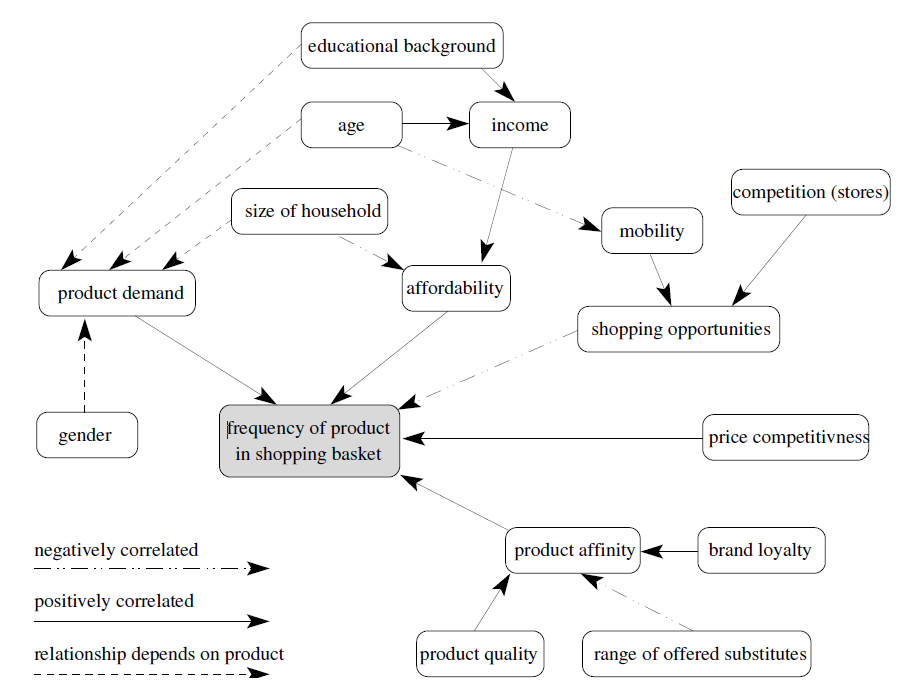
\includegraphics[width=\textwidth]{img/cognitive-map.PNG}

\subsection{Analysis goals}
Tasks of data mining are classification, regression, cluster analysis, finding associations, deviation analysis and so on.

The goals of analysis are to achieve/increase:

\begin{itemize}
	\item interpretability,
	\item reproduceability, stability,
	\item model flexibility, adequacy,
	\item runtime,
	\item interestingness
\end{itemize}

\subsection{Questions in data understanding}
\textbf{Goals}: Gain insight to data w.r.t to project goals and general.

Questions to be answered:
\begin{itemize}
	\item Attributes?
	\item Data quality?
	\item Visualization is helping?
	\item Attributes correlated?
	\item Outliers?
	\item Missing values?
\end{itemize}

\subsubsection{Attributes}
In a table a row is called instance, record, DO and columns are called attributes, features or variables.

\textbf{Types:} Categorical, Ordinal, Numerical, Discrete, Continuous.

\subsubsection{Data quality}
\textbf{Accuracy:} Closeness between values in data and true values, but:
\begin{itemize}
	\item low for numerical because of noisy measurments, limited precision, wrong measurements, transposition of digits
	\item low for categorical attributes because of erroneous entries and typos.
\end{itemize}

\textbf{Other factors:}
\begin{description}
	\item[Syntactic accuracy] Entry not in domain
	\item[Semantic accuracy] Entry in domain but not correct
	\item[Completeness] Entry not correct although belonging to domain (Missing rows e.g.)
	\item[Unbalanced data] Biased towards one type of record
	\item[Timeliness] Data up to date?
\end{description}

\subsection{Visualization}
\begin{tabular}{|c|c|p{7cm}|}
\hline 
\textbf{Type} & \textbf{Usage} & \textbf{Note} \\ 
\hline 
\textbf{Bar chart} & Frequencies & • \\ 
\hline 
\textbf{Histogram} & Frequency distribution & Number of bins $k = \log_2(n) + 1$ \\ 
\hline 
\textbf{Boxplot} & Shows distribution & Hisker: 1.5 iqr \\ 
\hline 
\textbf{Scatter} & Can help finding clusters and so on & Multi-dimensional mapping of data to two-dimensional plots \\ 
\hline 
\end{tabular} 

\subsection{Correlation analysis}
Trying to find similiar behaviour between two attributes.

\subsubsection{Pearsons correlation coefficient}
Measure for a linear relationship between two numerical attributes X and Y

\begin{center}
	$r_{xy} = \dfrac{\sum_{i=1}^n (x_i - \overline{x}) (y_i - \overline{y})}{(n-1) s_x s_y}$
\end{center}
The larger the absolute value is, the stronger the linear relationship is. If $\mid r_{xy} \mid = 1$ the values are exactly on one line.

\subsubsection{Rank correlation coefficients}
Pearson won't recognize monotone functional relationships but rank correlation coeffcients do, by ignoring the exact numerical values.
Only the order of the values is acknowleged.\\

\textbf{Spearman:} $\rho = 1 - 6\dfrac{\sum_{i=1}^n (r(x_1) - r(y_i))^2}{n(n^2-1)}$

\subsection{Outlier detection}
\textbf{Causes for outliers}: Data quality and exceptional situations.

\textbf{Handling:} If coming from big data sets they should be excluded from analysis even if the measurements were correct.
\subsubsection{Single attributes}
\begin{tabular}{|c|p{3cm}|c|p{6cm}|}
\hline 
\textbf{Type} & \textbf{Outlier?} & \textbf{Example} & \textbf{Goal} \\ 
\hline 
Categorical & Low/High frequencies for value & Automatic control system & Classifier to classify parts as correct or with failures based on measurements. Correct parts frequency might be to high so that failures might be considered outliers. \\ 
\hline 
Numerical & Extremly high or low values w.r.t. the other values & • & • \\ 
\hline 
\end{tabular} 

\subsection{Checklist for data understanding}
\begin{itemize}
	\item Determine quality of data
	\item Find outliers
	\item Detect and examine missing values (possibly default values!)
	\item Discover new or confirm expected dependencies or correlations between attributes
	\item Check specific application dependent assumptions
	\item Compare statistics and behaviour
	\item \textbf{Must Do! } Check distribution for each attribute
	\item \textbf{and!} check correlations or dependencies pairwise
\end{itemize}

\subsection{Multi-dimensional scaling (MDS)}
Only positions data points in low-dimensional space and uses distances between high dimensional data points as structure preservation.

\textbf{Input:} $(x_1, ..., x_2)$ with $x_i \in \mathbb{R}^d \rightarrow X$\\
\textbf{Output:} $(p_1, ..., p_n)$ with $p_io \in \mathbb{R}^q \rightarrow Y$, usually $q = 2$ or $q = 3$\\
\textbf{Goal:} Define $p_i$ for each record $x_i$ so that the distances are roughly the same.\\

\textbf{Distance requirement:}
\begin{itemize}
	\item non-negative: $d_{ij}^X \geq 0$
	\item symmetric: $d_{ij}^X = d_{ji}^X$
	\item diagonal should be zero: $d_{ii}^X = 0$
\end{itemize}

\subsubsection{Objective functions}
\textbf{Absolute squared error}: $E_0 = \sum_{i=1}^n \sum_{j=i+1}^n (d_{ij}^Y - d_{ij}^X)^2$\\
\textbf{Normalised absolute squared error}: $E_1 = \dfrac{1}{\sum_{i=1}^n \sum_{j=i+1}^n (d_{ij}^X)^2}\sum_{i=1}^n \sum_{j=i+1}^n (d_{ij}^Y - d_{ij}^X)^2$\\

The normalization factor $\dfrac{1}{\sum_{i=1}^n \sum_{j=i+1}^n (d_{ij}^X)^2}$ does not have an influence on the location of the minimum. Unlike $E_0$, $E_1$ does not depend on the number of data object and the magnitude of the original distances.\\

\textbf{Relative squared error:} $E_2 = \sum_{i=1}^n \sum_{j=i+1}^n \left( \dfrac{d_{ij}^Y - d_{ij}^X}{d_{ij}^X} \right)^2$\\
\textbf{Mixture of $E_0$ and $E_2$ (Sammon mapping):} $E_3 = \dfrac{1}{\sum_{i=1}^n \sum_{j=i+1}^n d_{ij}^X} \sum_{i=1}^n \sum_{j=i+1}^n \dfrac{(d_{ij}^Y - d_{ij}^X)^2}{d_{ij}^X}$

\subsubsection{Gradient descend method}
\begin{enumerate}
	\item Start with an arbitrary initial solution $x_0$
	\item Compute the gradient of $f$ at $x_0$\\
			Gradient is the vector for partial derivatives
	\item From $x_0$ go a fixed step width in the opposite direction of the gradient to find the next solution
	\item Continue iteratively..
\end{enumerate}

\subsubsection{Gradient for $E_1$}
$\frac{\eth E_1}{\eth y_k} = \dfrac{2}{\sum_{i=1}^n \sum_{j=i+1}^n (d_{ij}^X)^2} \sum_{j \neq k} (d_{kj}^Y - d_{kj}^X) \frac{y_k - y_j}{d_{kj}^Y}$

where

$\frac{\eth d_{ij}^Y}{\eth y_k} = \frac{\eth}{\eth y_k} \|y_i - y_j \| = \left\lbrace \begin{array}{ll}
	\frac{y_k - y_j}{d_{kj}^Y} & i = k, \\
	0 & otherwise
\end{array}\right.$\\

For the algorithm on how to use gradient descend on mds please see LS 78 in L02.

\section{Version Space}
\subsection{Inductive Learningg}
In inductive learning, \textbf{general} hypotheses are being introduced approximating a target function on the instance space from specific training data.

\textbf{Assumption:} Approximating a target function over the training data, will approximate the target function over the unobserved instances aswell.

\subsection{Concept learning}
Approximate target function c (characteristic function) using the attributes to distinguish instances (not) belonging to the concept.

The training data consists of positive and negative examples of the concept.

\textbf{Example Concept:} days on which aldo enjoys water sports..

Enjoying water sports is a binary attribute that can either be true or false, determining if the instance is a positive or a negative example.

\textbf{Formal:} $h : X \in \{0,1\}$ induced from $H$ so that $h(x) = c(x) \forall x \in D, D $ is the trainingset.

Possible values are either specific (water = warm), "don't care" = ? or no value allowed = $\emptyset$.

\subsection{Ordering hypothesis space}
If a function $h_j$ is more general than a function $h_k$ then it covers more instances than $h_j$. Formally if an instance is classified positive by $h_j$ it is implied that it also is classified positive by $h_k$.

\subsection{Searching hypothesis space}
Since exhaustive search is not possible in real life applications (due to huge aounts of data) the ordering of hypotheis has to be exploited such that searching is possible.

\textbf{Bottom-up} starting with general hypotheses $\rightarrow$ specialize

\textbf{Top-down} starting with specialized hypotheses $\rightarrow$ generalize

\subsubsection{Find-S}
Finds a maximally specific hypothesis..

Algorithm: Init \textit{h} to most specific hypothesis H

\begin{shadedSmallerPadding}
\begin{algorithm}[H]
	\caption{Find-S Algorithm}
	\SetAlgoLined
	\ForEach{positive training instance x}{
		\ForEach{attribute constraint $a_i$ in h}{
			\eIf{the contraint $a_i$ in h is satisfied by x}{do nothing}
				{generalize $a_i$ w.r.t. order until $a_i$ is satisfied by x}
		}
	}
			
		
\end{algorithm}

\textbf{Example:}

$x_1 = <Sunny,Warm,Normal,Strong,Warm,Same> +$\\
$x_2 = <Sunny,Warm,High,Strong,Warm,Same> +$ \\
$x_3 = <Rainy,Cold,High,Strong,Warm,Change> -$ \\
$x_4 = <Sunny,Warm,High,Strong,Cool,Change> +$\\
$h_0 = <\emptyset,\emptyset,\emptyset,\emptyset,\emptyset,\emptyset>$\\
$h_1 = <Sunny,Warm,Normal,Strong,Warm,Same>$\\
$h_{2,3} = <Sunny,Warm,?,Strong,Warm,Same>$\\
$h_4 = <Sunny,Warm,?,Strong,?,?>$
\end{shadedSmallerPadding}

\textbf{Pros:} Very efficient

\textbf{Cons:} Not complete (ignores negative examples)

\textbf{Questions:} Complexity? Multiple spec. hypo.? Why most spec. hypo?

\subsection{Definitions}

\textbf{Consistent:} $h$ is consistent with $D$ of $C$ if $h(x) = c(X)$ for each $<x, c(x)>$ in $D$, $D$ set of training examples.

\textbf{Version Space:} $VS_{H,D}$ w.r.t. $H, D$ is the subset of $H$ consistent with all training examples: $VS_{H,D} = \{h\in H \mid consistent(h,D)\}$

\textbf{General Boundary:} $G$ of $VS_{H,D}$ is the set of its maximally general members.

\textbf{Specific Boundary:} $S$ of $VS_{H,D}$ is the set of its maximally specific members.

\textit{Every member of $VS$ lies within these boundaries...}

\subsection{Candidate Elimination Algorithm}
Intialize $S$ and $G$..
\begin{algorithm}
\caption{Candidate Elimination Algorithm}
	\SetAlgoLined
	\ForEach{training example $d$}{
		\eIf{$d$ is positive example}{
			remove from $G$ any $h$ that is inconsistent with $d$\;
			\ForEach{$s \in S$ that is not consistent with $d$}{
				remove $s$ from $S$\;
				add to $S$ all minimal generalizations $h$ of $s$ such that\\
				(1) $h$ is consistent with $d$ and\\
				(2) some member of $G$ is more general than $h$
				\;
				remove from $S$ any $h$ that is more general than another $h \in S$\;
			}
		}
		{
			remove from $S$ any $h$ that is inconsistent with $d$\;
			\ForEach{$g \in G$ that is not consistent with $d$}{
				remove $g$ from $G$\;
				add to $G$ all minimal specializations $h$ of $g$ such that\\
				(1) $h$ is consistent with $d$ and\\
				(2) some member of $S$ is more specific than $h$
				\;
				remove from $G$ any $h$ that is less general than another $h \in G$\;
			}
		}
	}
\end{algorithm}

For an example see LS 161-163 in 1x1 all.

\textbf{Pros:} Considers negative examples, finds all consistent $h \in H$, can determine confidence, can detect inconsistencies

\textbf{Cons:} Not very efficient

\subsection{Unbiased learner}
\textbf{Why?: } Simple disjunctions cannot be represented so far.

H is chosen so that every possible of X with $|X| = 96$ is included, so that it surely contains any target concept.

\textbf{Inductive bias:} If it's too vague you can't generalize well, if it's too strict there is no consistent hypothesis. Use domain knowledge to choose an appropriate inductive bias..

\subsection{Concept learner discussion}
\textbf{Cons:}
\begin{itemize}
	\item can't handle inconsistent training data
	\item one ring to rule them all
	\item overfit of training data
\end{itemize}

\subsection{Validation of models}
Use a separate data set to evalute the generalization ability of the learned model

\section{Data preparation}
\subsection{Feature construction \& selection}
\textbf{Construction} of more useful attributes out of given attributes, e.g. the efficency of a worker based on his time to get a job done.\\
\textbf{Selection} of a subset of attributes that is as small as possible but still sufficient enough for data analysis.

\textbf{Techniques:}
\begin{itemize}
	\item Top-ranked features (best evaluation)
	\item Top-ranked subset (Best performance subset, requires exhaustive search)
	\item Forward (Start empty, add one by one, always choose best fitting feature)
	\item Backward elimination (eliminate features with smallest decrease in performance)
\end{itemize}

\subsection{Record selection}
Pros for subsampling: Faster computation, Cross-Validation, Timeliness, Representativeness, Rare events...

\subsection{Data cleansing}
Detecting, correcting and removing inaccurate, incorrect, incomplete records from a data set.

\subsection{Improve data quality}
\begin{itemize}
	\item Capital letters to handle case sensitivity
	\item Remove spaces / nonprints
	\item Format numbers, date and time
	\item Split mixed fields
	\item Spell checker usage to find typos
	\item Replace abbreviations or vice versa
	\item Normalize addresses, names, surname, forename (everything there is)
	\item Convert numerical values to standard units
	\item Use dictionaries
\end{itemize}

\subsection{Missing value}
\begin{itemize}
	\item ignore/delete
	\item imputate (replace by estimate)
	\item default value for missing values
\end{itemize}

\subsection{Transformation of data}
\textbf{Transformation of categorical data to numerical:}

If binary (male, female) convert to 0 and 1. If ordinal just assign the value in order. If categorical with more than two values, create binary attributes for each possible value.

\textbf{Transformation from numerical to categorical data:}
\begin{description}
	\item[Equi-width] Splits into intervals
	\item[Equi-frequency] Splits into intervals so the bins are the same size
	\item[V-optimal] ??
	\item[Minimal entropy] Well..
\end{description}

\subsection{Normalization/Standardization}
\textbf{min-max:}\\
$n: dom(X) \rightarrow [0,1], x \rightarrow \dfrac{x - min_x}{max_x - min_x}$

\textbf{z-score:}\\ $s: dom(X) \rightarrow \mathbb{R}, x \rightarrow \dfrac{x- \hat{\mu_x}}{\hat{\sigma}}$

\textbf{decimal scaling:}\\
s is the smallest int value larger than $log_{10} max_x$\\
$d: dom(X) \rightarrow [0,1], x \rightarrow \frac{x}{10^s}$

\subsection{PCA}
\textbf{Performing a pca:}
Constructs a projection to lower-dimensional space by using the variance as structure preservation criterion.

\begin{enumerate}
	\item Subtract mean from each value
	\item Calclate covariance matrix
	\item Calculate eigenvectors and eigenvalues
	\item Choose eigenvectors and eigenvalues by significance
	\item Apply to data
\end{enumerate}

\section{Modeling}
\textbf{The four steps of modeling:}
\begin{enumerate}
	\item Select model class
	\item Select score function
	\item Apply algorithm
	\item Validate results
\end{enumerate}

\subsection{Model class}
Form and structure of the analysis result. E.g. regression, statistical values, rules..

\textbf{Requirements:}
\begin{description}
	\item[Simplicity] Simplest model that still explains the data (easier to understand, lower complexity, avoid overfitting)
	\item[Interpretability] Black box often not a good choice, but often a good accuracy (neural networks)
\end{description}

\subsection{Global and local models}
\textbf{Global models} provide a description for the whole data set (Regressions).

\textbf{Local models} concentrate on subsets of the data.

\subsection{Fitting criteria and score function}
\textbf{Goal:} Find objective function to evalute your model. Is used to find the best model.

\textbf{Example:} The means squared and mean absolute error functions are such score functions to evaluate the model. They'll tell if the error rate of your predictions are low or high.

\textbf{Mean squared:} $f(D) = \frac{1}{n} \sum_1^n(y_i - \mathcal{M}(x_i))^2$

\textbf{Mean absolute:} $f(D) = \frac{1}{n} \sum_1^n|(y_i - \mathcal{M}(x_i))|$

\subsection{Error functions for classification}
Common error function \textbf{misclassification rate}: $\frac{\#wrong \ classified}{\#total \ classified}$

\textit{Low misclassification rate doesn't necessarily tell anything about the qality of the classifier}

\textbf{Cost Matrix}
Another more general approach than misclassification rate is the cost matrix.

\begin{tabular}{|c|c|c|}
\hline true class & OK & broken \\ 
\hline OK & 0 & $c_1$ \\ 
\hline broken & $c_2$ & 0 \\ 
\hline 
\end{tabular} 

This method can be applied on a various number of classes!

The expected losst can be calculated using $loss(c_i | E) = \sum_1^m P(c_j | E) c_{ji}$ and can then be minimized, wheras $E$ are the observed values by the predictor attributes and $P(c_j | E)$ is the probability that the class is $c_j$ w.r.t. $E$.

For an example see LS 225 in 1x1 all.

\subsection{Algorithms for model fitting}
Objective function doesn't tell if a model is good. That's why optimisation algorithms to find the best or at least a good model are needed.
\subsubsection{Closed form solutions}
An example is \textbf{to find a regression line} that minimizes the mean square error.

The formulae is:

$a = \dfrac{n \sum_1^n x_i y_i . (\sum_1^n x_i) (\sum_1^n y_i)}{n \sum_1^n x_i^2 - (\sum_1^n x_i)^2}$

$b = \overline{y} - a\overline{x}$\\

\subsubsection{Other solutions}

\textbf{For differntiable} functions, gradient methods can be applied. As seen in LS230 1x1 these methods will only find local optima an the parameters have to be optimized within every iteration.

\textbf{For discrete} problems with finite search space, combinatorial optimaization strategies are needed. It is possible to search a finite domain $\mathcal{M}$, but in most cases $\mathcal{M}$ is too large.

E.g. in a set of 1000 items the number of nonempty subsets isw over $10^{300}$.

\textbf{There are a couple of heuristic strategies that can be applied, such as:}

\textbf{Random search} - very inefficient\\
\textbf{Greedy strategies} - Iterative improvements such as gradient method, hillclimbing. Solutions can be found quickly but also can get stuck on local optima...\\
\textbf{Simulated annealing} - Mix between the previous, modified version of hillclimbing, sometimes works out worse (low probability) but gets better with every iteration step...\\
\textbf{Evolutionary algorithms} - Multiple solutions are being sed to search space in parallel and efficiently..\\
\textbf{Alternating optimisation} - Disjuncts parameters into subsets an calculates analytical solutions for every disjunction and iterates scheme until convergence.

\subsection{Model error}
4 possible origins: Experimental error, Sample error, Model error, Algorithmic error..

\subsubsection{Experimental error}
Also called bayes error when associated with classifications problems.

\textbf{ROC curves:} the higher the are under curve (AUC) the better..

\textbf{Confusion matrix} is a table where the true and the predicted classes are listed.

\subsubsection{Sample error}
Can come from falsy measurements and manipulations..

\subsubsection{Model error}
Simpler model -> bigger error\\
More comlex -> chance of overfitting and larger error on new data
Type of model -> different "fit" to data

\subsubsection{Algorithmic error}
E.g. gradient descend -> local minima, randomized method -> too much randomness..

\subsection{Machine learning bias and variance}
Machine learners are treating model and algorithmic error as bias whereas intrinsic and sample error are variance.

\textbf{One cannot simply learn without a bias!}

Also the error for unseen data is most commonly bigger than with training data.. That's why training and test data are used (typically 2/3 training and 1/3 test data).

There are different splitting strategies:

\textbf{Random}

\textbf{Stratification} - i.e. distribuion of a class should remain

\subsection{Validation of models}
$T = T_{train} \cup T_{eval}$ and
$\emptyset = T_{train} \cap T_{eval}$

$P(E) = \dfrac{\sum_{x \in T_{eval}} g(H(x), C(x))}{|T_{eval}|}$

with

$g(x,y) = 1$ if $x = y$ and $g(x,y) = 0$ if $x \neq y$..

this is the rate where the model classified correctly on $T_{eval}$

\subsubsection{Cross-Validation}
Data gets split multiple times. Later on either a combination or the best model is used.

\textbf{K-Fold Cross-Validation} divides the data into k subsets, where the average of the k model error is supposed as the model error..

\textbf{Leave-One-Out Methode} is for small data sets and uses everything except for one data point for training. The single data point is used for testing..

\subsubsection{Bootstraping}
\textbf{Goal:} Draw samples multiple times

\begin{enumerate}
	\item Draw k bootstrap samples
	\item Learn model on each sample
	\item Calculate mean and standard deviation
	\item Small standard deviation supports model
\end{enumerate}

\textbf{Bagging} means the use of bootstrapping to improve results

\textbf{Averaging} k sets of parameters will give the final parameters

\subsection{Minimum description length principle}
\textbf{Idea:} Look at the model as a way of data compression, which means you nead a \textbf{decompression rule} and \textbf{compressed data}.

\textbf{Quality} is measured by the number of bits needed to code the above. \textbf{The simplest cases} are compressed data size = 1 and decompression rule size = 1.

\textbf{Example:} Coding of decimals is restricted to two digits and sig is ignored. 0.73 $\rightarrow$ 37, 1.23 $\rightarrow$ 321 and -0.06 $\rightarrow$ 6..

If you consider the error a function creates e.g. for x = 1 and error = 0.73 you have to sum up all digits created by the mdl. Pick the model which sum is the lowest. You also have to consider the digits calculated for the model values aswell e.g. y = 1.14 + 0.19x resolves in 5.

\section{Clustering}
\subsection{Finding patterns}
is an exploratory data analysis task. Not target attribute as in supervised learning. 

\textbf{Methods for finding patterns:} Clustering and association rules.

\subsection{What is a cluster}
A cluster is a group of similiar objects or more formally:

\begin{shadedSmallerPadding}
	Clustering identifies a finite set of categories $C_1 ... C_k$ in a dataset so that objects in $C_i$ are as similiar as possible.
	
	\textbf{Properties:} Different sizes, shapes, densities, form hierarchy, oberlap or be disjoint.
\end{shadedSmallerPadding}

\textbf{Goals of cluster analysis:}

For different tasks different goals are set:

\begin{description}
	\item[Data understanding] Find natural clusters, describe properties
	\item[Data Class Ident.] Useful and suitable groupings
	\item[Data reduction] Representatives for homogenous groups
	\item[Outlier detection] Unusual objects
	\item[Noise detection] Find random perturbations in the data
\end{description}

\subsection{Similarity Measures}
\subsubsection{Numerical attributes}
Dissimilarities between numerical attributes can be calculated using different formulas:

\begin{tabular}{|c|c|}
\hline 
Minkowski & $d_p(x,y) = \sqrt[p]{\sum_1^n|x_i - y_i|^p}$ \\ 
\hline 
Euclidean & $d_E(x,y) = \square{\sum_1^n (x_i - y_i)^2}$ \\ 
\hline 
Manhatten & $d_M(x,y) = \sum_1^n |x_i - y_i|$ \\ 
\hline 
Tschebyschew & $d_\infty(x,y) = max\{\|x_1 - y_1|, ..., |x_n - y_n| \}$ \\ 
\hline 
Cosine & $d_C(x,y) = 1 - \dfrac{x^Ty}{\parallel x \parallel \parallel y \parallel}$ \\ 
\hline 
Tanimoto & $d_T(x,y) = 1 - \dfrac{x^Ty}{\parallel x \parallel^2 + \parallel y \parallel^2 - x^Ty}$ \\ 
\hline 
Pearson & Euclidean of z-score \\ 
\hline 
\end{tabular} 

\subsubsection{Binary attributes}
Can be used to interpret a property as being abscent or not being abscent.

\begin{tabular}{|c|c|c|}
\hline 
 & binary attributes & sets of properties \\ 
\hline 
simple match & $d_S = 1 - \frac{b+n}{b+n+x}$ & \\ 
\hline 
Russel and Rao & $d_R = 1 - \frac{b}{b+n+x}$ & $1 - \frac{|X \cap Y|}{ |\Omega|}$ \\ 
\hline 
Jaccard & $d_J = 1 - \frac{b}{b+x}$ & $1 - \frac{|X \cap Y|}{ |X \cup Y|}$ \\ 
\hline 
Dice & $d_D = 1 - \frac{2b}{2b+x}$ &  $1 - \frac{2|X \cap Y|}{ |X| + |Y|}$ \\ 
\hline 
\end{tabular}

where \textbf{b} holds in both records, \textbf{n} holds in none and \textbf{x} holds in one.

\textbf{Example:}

\textbf{101000} and \textbf{111000} with b=2, n=3, x=1 and corresponding $d_s = 0.166, d_R = 0.66, d_J = 0,33, d_D = 0.2$.

\subsubsection{Nominal attributes}
A nominal attribute can be transformed into a set of binary atttributes, which then can be use to apply binary attribute methods.

\subsection{Hierarichal Clustering}
\textbf{AGNES} (Aglomerative Nesting) is a bottom-up method to cluster hierarichly.

\textbf{DIANA} (Divisive analysis) is a top-down method to cluster hierarichly.

This method is very expensive and needs to check $2^(n-1)-1$ in the first step!

\textbf{To decide which objects} belong to the same cluster similarity measures have to be calculated, for which a matrix is created and should satisfy

\begin{itemize}
	\item $d_{i,j} \geq 0$
	\item $d_{i,i} = 0$
	\item $d_{i,j} = d_{j,i}$
\end{itemize}

Also the \textbf{triangle inequality} $d_{i,k} \leq d_{i,j} + d_{j,k}$.

\subsubsection{AGNES Algorithm}
\begin{algorithm}
	\SetAlgoLined
	
	Start with n clusters, each object is a single cluster\;
	\While{More than one cluster left}{
		Reduce the number by joining the most similiar\;
	}
\end{algorithm}

\subsubsection{Distance between clusters}
\begin{description}
	\item[Centroid] Distance between mean value vectors (meaning the mean of all members in the clusters!)
	\item[Average linkage] Average dissimilarity between all pairs of points of the two clusters, compact clusters as result
	\item[Single linkage] Dissimilarity between two most similar objects of t he two clusters counts, good to follow chains
	\item[Complete linkage] Dissimilarity between two most d objects of t he two clusters counts, compact clusters as result
\end{description}

\textbf{How to calculated distances between clusters for each method?}
\begin{description}
	\item[Centroid] unclear see ls......
	\item[Average linkage] unclear see ls ...
	\item[Single linkage] see ls very easy
	\item[Complete linkage] see ls very easy
\end{description}

\subsubsection{Choosing the right cluster}
\begin{description}
	\item[Simple] define minimum distance
	\item[Visual] Find a good cut level visualy
	\item[Sophisticated] analyze distances between clusters in each step. try to find distance which is considerably higher than in previous steps.
\end{description}

\subsubsection{Heatmaps}

Visual representation to underline the values of attributes in a dendrogram using colors.

\subsubsection{DIANA}
Agglomerative has quad. complexity in each step whereas diana has $2^{n-1}-1$ possible splits in the first step where n is the number of the data objects.

\subsection{Prototype based clustering}
\subsubsection{k-Means}
\textbf{Pseudo-Algorithm}
\begin{enumerate}
	\item Choose k clusters
	\item Init. randomly
	\item Assign data point to nearest cluster center
	\item Compute new center clusters and start 3. again until either no changes ot number of iterations have been exceeded.
\end{enumerate}

\textbf{Pros:} Efficient, Finds cluster centers if shapes are concave and clusters have reasonable distance to one another. Simple implementation.

\textbf{Cons:} Won't work on convex shapes and is sensitive to initial positions. Also may be stuck at a local minimum. Only working on numerical data.

\subsection{Quality measures}
\begin{description}
	\item[Centroid $\mu_C$] mean vector of objects in Cluster C
	\item[Within Cluster Variation] $TD^2(C) = \sum_{p \in C} dist(p, \mu_C)^2$\\
	$TD^2 = \sum_{i=1}^k TD^2(C_i)$
	\item[Between Cluster Variation] $BC^2 = \sum_{j=1}^{k} \sum_{i=1}^{k} dist(\mu_i, \mu_j)^2$
	
	\item[Clustering Quality] $CQ = \dfrac{BC^2}{TD^2}$
\end{description}

\subsubsection{Silhouette-Coefficient}
\begin{itemize}
	\item a(x) - distance from x to own cluster
	\item b(x) - distance from x to next best cluster
	\item silhouette $s(x) = \dfrac{b(x) - a(x)}{max\{a(x), b(x)\}}$
\end{itemize}

\subsection{Gaussian mixture models}
Data samples are generated out of normal distributions. Analyze and find the paramters for the NV.

\textbf{Algorithm:} EM Clustering

Parameters are being estimated..

\subsection{Density Based Clustering}
\textbf{Pro:} Often yields best results on numerical data.

\textbf{Idea:} High density in region = Cluster

\subsubsection{DBSCAN}
\begin{enumerate}
	\item Find data point in which $\epsilon$-neighborhood are at least \textbf{l} other points
	\item Expand neighbourhood as long as criterion satisfied
	\item Continue without considering this cluster
\end{enumerate}

\section{Association Rules}
\textbf{Support of itemset:} Frequency it shows up

\textbf{Support of AR $X \rightarrow Y$:} Common - support of $X \cup Y$, Plausible - support of X

\textbf{Confidence:} Support $X\cup Y$ divided by support of X

\subsection{Searching frequent item sets}
\subsubsection{Properties of itemsets}
\textbf{If an item set is extended, its support cannot increase.}

\textbf{No superset of an infrequent item set can be frequent. - Apriori Priority}

\subsubsection{Apriori algorithm}
\begin{itemize}
	\item Determine support of 1-element itemsets
	\item discard infrequents
	\item ...
	\item Form candidate item sets k items, discard infrequents
\end{itemize}

This is based on two main steps: candidate generation and pruning.

see ls for all 3 algorithms assocated with this matter.

\subsubsection{Searching wth unique parents}
\textbf{Principles:}
\begin{itemize}
	\item Base loop: Traverse 1-element item sets (parent is empty set) \\
		  recursively process frequent ones
	\item Recursive processing: Generate extensions of unique parent I and process it recursively if it is frequent, otherwise discard..
\end{itemize}

\textbf{Assigning unique parents:}
All possible parents of an item set $I$ are its maximal proper subsets.

\subsection{Canonical Forms}
Lexicographically smallest word is the canonical form!

The \textbf{canonical parent} of an itemset is the itemset described by the longest proper prefix and is equivalent to $p_c(I) = I - \{max a\}$

\textbf{Recursive processing:}
Consider an itemset I, which is extended by all items. If the last letter of the canonical representation of the newly formed set is the item added to I continue with the new set as done with I otherwise discard the new set.

\subsubsection{Prefix property}
The previously shown item set coding scheme has the prefix property: \textbf{The longest proper prefix of the canonical code word of any item set is a canonical code word itself.}

E.g. $\{a,b,c,d\} \rightarrow \{a,b,c\}$

\textbf{Every prefix of a canonical code word is a canonical word itself......}

\subsubsection{Searching with the prefix property}
The general recursive processing scheme with canonical forms requires to construct canonical code words of each created item set to decide whether to apply further. This is simplified by the prefix property scheme.

What actually only has to be checked is, whether or not the resulting code word is canonical itself or not, otherwise discard right away.

\textbf{Advantage:} Faster than constructing it from scratch.

\textbf{Principle Algorithm based on prefix property:}
\begin{description}
\item[Base loop] Traverse all possible items (already canonical, not?)\\
	Recursively apply the new scheme on those items that are frequent
	
\item[Recursive Processig] $\forall$: Create all extensions by one item\\
	If extended word canonical AND frequent, process recursively..
\end{description}

This scheme can be applied on the apriori algorithm during candidate generation and leads to a resonable faster runtime!

The final algorithm based on canonical forms is as follows:

\begin{description}
\item[Base loop] SAME
\item[Recursive processing] for canonical word of a frequent item set, do:\\
	Generate all possible extensions by one item (insert last). If canonical and frequent process recursively (WHAT HAS CHANGED HERE?)
\end{description}

\subsection{Canonical parents and Prefix trees}
\begin{itemize}
\item itemsets that have same longest proper prefix are siblings
\item Also called trie (remember that for DL).
\item using merged sibilings results in a overviewable prefix tree
\end{itemize}

\subsubsection{Search tree pruning}
Search trees tend to get very large, pruning is needed:

\begin{description}
\item[Structural] canonical word based representation removes superfluouspaths
\item[Support based] Superset of infrequent itemsets can't be frequent
\item[Size based] Prune for certain depth
\end{description}

The structure of the (structurally pruned) prefix tree depends on the chosen order of the items $\rightarrow$ size and number of nodes influence the execution times of frequent item set mining algorithms considerably.

Heuristics for choosing an item order are usually based on conditional independence assumptions.

\subsubsection{Heuristics for Choosing the Item Order}
\textbf{Basic Idea:}

\textbf{FIS} consist of \textbf{FIS}:
\begin{itemize}
	\item Sort items by support
	\item Sort descendingly: Prefix tree has fewer, but larger (meaning more siblings) nodes
	\item Sort ascendingly: Prefix tree has more, but smaller nodes..
\end{itemize}

\textbf{Extension of this idea:} Sort items w.r.t. sum of transaction sizes they appear in

\subsubsection{Searching the Prefix Tree Levelwise}
\textbf{Apriori idea:}

\begin{itemize}
	\item Check item sets in increasing size (levelwise)
	\item Canonical form should ensure that each candidate is generated at most once
	\item A priori pruning is then applied onto the generate levels (before the support of the itemsets has been determined)
	\item Representation of transactions: Array
	\item Support is calculated by checking if they are subsets of  transactions
\end{itemize}

\textbf{Node organization}
\begin{description}
	\item[Direct indexing] Node as vector of counters, fast access, high memory usage
	\item[Sorted Key-Value Pairs] Node as vector of item/counter pairs, binary search, not as fast but slower memory usage
	\item[Hash tables] Node as vector of item/counter pairs (closed hashing), faster access than binary search, higher memory usage
\end{description}

\section{Finding Explanations}
\subsection{Bayes}
\subsection{Regression}
\subsection{Decision Trees}
\subsection{Rule Learning}
\section{Predictors}
\subsection{Nearest Neighbor}
\subsection{Kernel / SVM}
\subsection{Meta Learning}

\end{document}


























